% Options for packages loaded elsewhere
\PassOptionsToPackage{unicode}{hyperref}
\PassOptionsToPackage{hyphens}{url}
\PassOptionsToPackage{dvipsnames,svgnames,x11names}{xcolor}
%
\documentclass[
  letterpaper,
  DIV=11,
  numbers=noendperiod]{scrartcl}

\usepackage{amsmath,amssymb}
\usepackage{iftex}
\ifPDFTeX
  \usepackage[T1]{fontenc}
  \usepackage[utf8]{inputenc}
  \usepackage{textcomp} % provide euro and other symbols
\else % if luatex or xetex
  \usepackage{unicode-math}
  \defaultfontfeatures{Scale=MatchLowercase}
  \defaultfontfeatures[\rmfamily]{Ligatures=TeX,Scale=1}
\fi
\usepackage{lmodern}
\ifPDFTeX\else  
    % xetex/luatex font selection
\fi
% Use upquote if available, for straight quotes in verbatim environments
\IfFileExists{upquote.sty}{\usepackage{upquote}}{}
\IfFileExists{microtype.sty}{% use microtype if available
  \usepackage[]{microtype}
  \UseMicrotypeSet[protrusion]{basicmath} % disable protrusion for tt fonts
}{}
\makeatletter
\@ifundefined{KOMAClassName}{% if non-KOMA class
  \IfFileExists{parskip.sty}{%
    \usepackage{parskip}
  }{% else
    \setlength{\parindent}{0pt}
    \setlength{\parskip}{6pt plus 2pt minus 1pt}}
}{% if KOMA class
  \KOMAoptions{parskip=half}}
\makeatother
\usepackage{xcolor}
\setlength{\emergencystretch}{3em} % prevent overfull lines
\setcounter{secnumdepth}{-\maxdimen} % remove section numbering
% Make \paragraph and \subparagraph free-standing
\ifx\paragraph\undefined\else
  \let\oldparagraph\paragraph
  \renewcommand{\paragraph}[1]{\oldparagraph{#1}\mbox{}}
\fi
\ifx\subparagraph\undefined\else
  \let\oldsubparagraph\subparagraph
  \renewcommand{\subparagraph}[1]{\oldsubparagraph{#1}\mbox{}}
\fi


\providecommand{\tightlist}{%
  \setlength{\itemsep}{0pt}\setlength{\parskip}{0pt}}\usepackage{longtable,booktabs,array}
\usepackage{calc} % for calculating minipage widths
% Correct order of tables after \paragraph or \subparagraph
\usepackage{etoolbox}
\makeatletter
\patchcmd\longtable{\par}{\if@noskipsec\mbox{}\fi\par}{}{}
\makeatother
% Allow footnotes in longtable head/foot
\IfFileExists{footnotehyper.sty}{\usepackage{footnotehyper}}{\usepackage{footnote}}
\makesavenoteenv{longtable}
\usepackage{graphicx}
\makeatletter
\def\maxwidth{\ifdim\Gin@nat@width>\linewidth\linewidth\else\Gin@nat@width\fi}
\def\maxheight{\ifdim\Gin@nat@height>\textheight\textheight\else\Gin@nat@height\fi}
\makeatother
% Scale images if necessary, so that they will not overflow the page
% margins by default, and it is still possible to overwrite the defaults
% using explicit options in \includegraphics[width, height, ...]{}
\setkeys{Gin}{width=\maxwidth,height=\maxheight,keepaspectratio}
% Set default figure placement to htbp
\makeatletter
\def\fps@figure{htbp}
\makeatother

\usepackage{pexample}
\usepackage{easy-todo}
\KOMAoption{captions}{tableheading}
\makeatletter
\@ifpackageloaded{caption}{}{\usepackage{caption}}
\AtBeginDocument{%
\ifdefined\contentsname
  \renewcommand*\contentsname{Table of contents}
\else
  \newcommand\contentsname{Table of contents}
\fi
\ifdefined\listfigurename
  \renewcommand*\listfigurename{List of Figures}
\else
  \newcommand\listfigurename{List of Figures}
\fi
\ifdefined\listtablename
  \renewcommand*\listtablename{List of Tables}
\else
  \newcommand\listtablename{List of Tables}
\fi
\ifdefined\figurename
  \renewcommand*\figurename{Figure}
\else
  \newcommand\figurename{Figure}
\fi
\ifdefined\tablename
  \renewcommand*\tablename{Table}
\else
  \newcommand\tablename{Table}
\fi
}
\@ifpackageloaded{float}{}{\usepackage{float}}
\floatstyle{ruled}
\@ifundefined{c@chapter}{\newfloat{codelisting}{h}{lop}}{\newfloat{codelisting}{h}{lop}[chapter]}
\floatname{codelisting}{Listing}
\newcommand*\listoflistings{\listof{codelisting}{List of Listings}}
\makeatother
\makeatletter
\makeatother
\makeatletter
\@ifpackageloaded{caption}{}{\usepackage{caption}}
\@ifpackageloaded{subcaption}{}{\usepackage{subcaption}}
\makeatother
\ifLuaTeX
  \usepackage{selnolig}  % disable illegal ligatures
\fi
\usepackage{bookmark}

\IfFileExists{xurl.sty}{\usepackage{xurl}}{} % add URL line breaks if available
\urlstyle{same} % disable monospaced font for URLs
\hypersetup{
  colorlinks=true,
  linkcolor={blue},
  filecolor={Maroon},
  citecolor={Blue},
  urlcolor={Blue},
  pdfcreator={LaTeX via pandoc}}

\author{}
\date{}

\begin{document}

\begin{document}    
\betterposter{
%%%%%%%% MAIN COLUMN

\maincolumn{
%%%% Main space

\textbf{We failed to detect a causal effect of FMD on CKD}. However, due to the \textbf{small number of relevant SNPs}, we had \textbf{limited power}. 
}{
%%%% Bottom space

%% QR code
\qrcode{img/qrcode}{img/smartphoneWhite}{
\textbf{Take a picture} to
\\download the full paper
}
% Smartphone icon
% Author: Freepik
% Retrieved from: https://www.flaticon.com/free-icon/smartphone_65680

%% Compact QR code (comment the previous command and uncomment this one to switch)
%\compactqrcode{img/qrcode}{
%\textbf{Take a picture} to
%\\download the full paper
%}

}

}{
%%%%%%%% LEFT COLUMN

\title{Assessing Evidence That Fibromuscular Dysplasia Causes Chronic Kidney Disease: A Two-Sample Mendelian Randomization Study}
\author{Frederick J. Boehm}
\author{Min-Lee Yang}
\author{Xiang Zhou}
\author{Santhi K. Ganesh}
\institution{University of Michigan}

\section{Introduction}
\textbf{Fibromuscular dysplasia (FMD)} is a systemic disease of artery walls that decreases target organ perfusion. 
Investigators have identified \textbf{chronic kidney disease (CKD)} as a possible consequence. 
% is there other evidence for this relationship? actual epidemiology studies??
% cite the actual case studies!!
\begin{center}
\includegraphics[width=\textwidth]{Fibromuscular.png}
\end{center}    

\begin{itemize} % perhaps add facts or evidence in itemized list below, to tie ckd to fmd
\item FMD often affects renal arteries \cite{olin2012united}.
\item FMD complications include stroke, dissection, \& aneurysm \cite{olin2012united}.
\end{itemize}

\section{Mendelian Randomization}


% https://media.springernature.com/full/springer-static/image/art%3A10.1038%2Fs41431-022-01038-5/MediaObjects/41431_2022_1038_Fig1_HTML.png?as=webp
    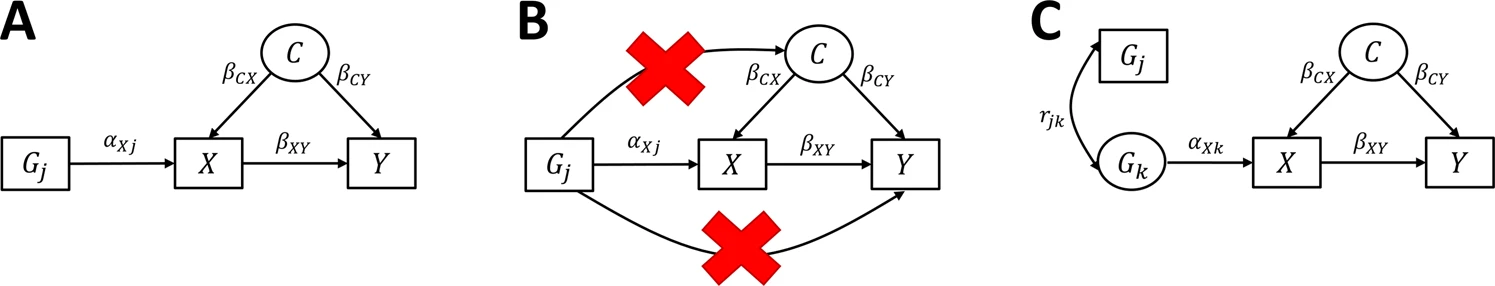
\includegraphics[width=\textwidth]{mr.png} % is this the figure that I want to use? 
    % Check the latest figures in teh Gen Epi letter about MR diagrams
    \cite{de2022understanding}




%% This fills the space between the content and the logo
\vfill

%% Institution logo

\includegraphics[width=\textwidth]{img/logo}\\

}{
%%%%%%%% RIGHT COLUMN
\section{Two-sample MR with GWAS Summary Statistics}
\begin{itemize}
\item FMD GWAS \cite{georges2021genetic}
\item CKD GWAS \cite{neale_lab_gwas}
\end{itemize}


\section{FMD GWAS Meta-analysis \cite{georges2021genetic}}
\begin{itemize}
\item Six case-control studies from USA and Europe  
\item 1556 cases \& 7100 controls  
\item Tested 5.5 million SNPs  
\item Identified four risk loci for FMD: \textit{PHACTR1, LRP1, LIMA1, ATP2B1}  
\end{itemize}
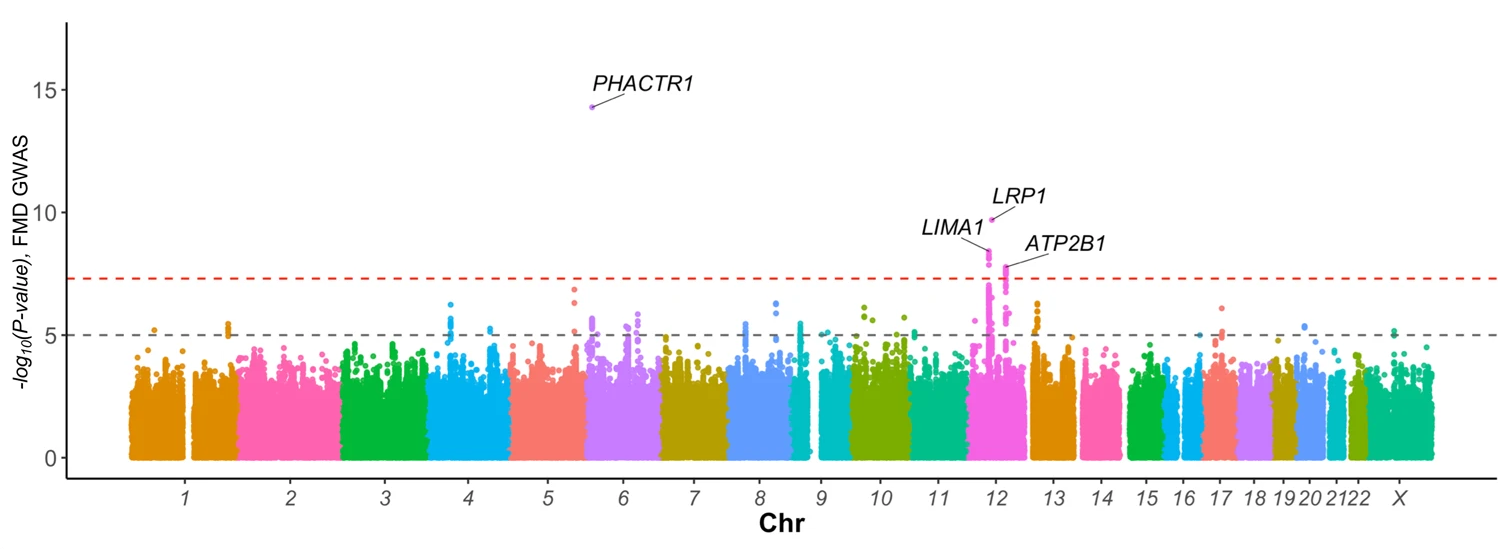
\includegraphics[width=\textwidth]{georges2021-Fig1.png} 




\section{CKD GWAS \cite{neale_lab_gwas}}
\begin{itemize}
\item 194,174 female UKB subjects -- check number of missing for this trait!
\end{itemize}


\section{MR Results}




\section{Conclusion}





\section{References}
\printbibliography[heading=none]


\section{Contact}
\textbf{Fred Boehm}\\
Email: frederick.boehm@gmail.com\\
Website: \url{https://fboehm.us}\\
Poster repository: \url{https://github.com/fboehm/statgen2024}


\section{Acknowledgements}
\textbf{Funding}: The National Institutes of Health (NIH) grant T32HL007853 to David J. Pinsky supported our research. The University of Michigan Postdoctoral Association supported our participation in STATGEN2024. 

}
\end{document}



\end{document}
